\section{Udvælgelse af gestik-par til pause og start}
\label{TestresultaterPauseStart}
%
Udvælgelsen af hvilket gestik-par, der skal knyttes til pause og start foretages på baggrund af testpersonernes udsagn. I \fullref{app:TestresultaterPauseDaarlig} analyseres testpersonernes respons i forhold til, hvilke gestik-par de mindst kan lide og på baggrund af den analyse ekskluderes gestik-par 2, gestik-par 3 og gestik-par 4 fra yderligere undersøgelser. Dette medfører at udvælgelsen af hvilket gestik-par, der skal knyttes til pause og start kun foretages på gestik-par 1, gestik-par 5, gestik-par 6 og gestik-par 7. Analysen bygger på testpersonernes respons til de tre spørgsmål: \textit{Hvordan vil du rangere de tre bedste gestikker?}, \textit{Hvorfor har du valgt netop de tre?} og \textit{Hvorfor har du rangeret dem, som du har?}, hvor testpersonernes samlede data er vedlagt i \autoref{app:NoterValgAfGestikker}.\blankline
%  
I nedenstående \autoref{tab:GestikParITopTrePause} fremgår samtlige testpersoners top tre rangering, hvor der ikke er taget forbehold for, hvorvidt testpersonerne har inkluderet et gestik-par, som der på baggrund af \fullref{app:TestresultaterPauseDaarlig} er blevet ekskluderet.
%
\begin{table}[H]
	\centering
	\begin{tabular}{ | p{3cm} | p{3cm} | p{3cm} | p{3cm} |}
	\hline
		 & 1. Plads & 2. Plads & 3. Plads \\ \hline
		Testperson 1 & Gestik-par 1 & Gestik-par 7 & Gestik-par 5 \\ \hline
		Testperson 2 & Gestik-par 7 & Gestik-par 6 & Gestik-par 1 \\ \hline
		Testperson 3 & Gestik-par 1 & Gestik-par 2 & Gestik-par 4 \\ \hline
		Testperson 4 & Gestik-par 1 & Gestik-par 5 & Gestik-par 7 \\ \hline
		Testperson 5 & Gestik-par 5 & Gestik-par 1 & Gestik-par 6 \\ \hline
		Testperson 6 & Gestik-par 1 & Gestik-par 5 & Gestik-par 7 \\ \hline 
		Testperson 7 & Gestik-par 5 & Gestik-par 2 & Gestik-par 6 \\ \hline
		Testperson 8 & Gestik-par 7 & Gestik-par 3 & Gestik-par 6 \\ \hline
		Testperson 9 & Gestik-par 7 & Gestik-par 1 & Gestik-par 6 \\ \hline
		Testperson 10 & Gestik-par 1 & Gestik-par 2 & Gestik-par 4 \\ \hline
		Testperson 11 & Gestik-par 5 & Gestik-par 7 & Gestik-par 6 \\ \hline
		Testperson 12 & Gestik-par 2 & Gestik-par 1 & Gestik-par 5 \\ \hline
		Testperson 13 & Gestik-par 6 & Gestik-par 3 & Gestik-par 5 \\ \hline
		Testperson 14 & Gestik-par 6 & Gestik-par 5 & Gestik-par 7 \\ \hline
		Testperson 15 & Gestik-par 1 & Gestik-par 4 & Gestik-par 5 \\ \hline
		Testperson 16 & Gestik-par 1 & Gestik-par 5 & Gestik-par 7 \\ \hline
		Testperson 17 & Gestik-par 1 & Gestik-par 5 & Gestik-par 7 \\ \hline
		Testperson 18 & Gestik-par 5 & Gestik-par 7 & Gestik-par 1 \\ \hline
	\end{tabular}
	\caption{Oversigt over samtlige testpersoners top tre i forbindelse med pause og start.}
	\label{tab:GestikParITopTrePause}
\end{table}
\noindent
%
Få at få et overblik over, hvor ofte de syv forskellige gestik-par individuelt indgår på enten en første, anden eller tredje plads i top tre rangeringen opstilles følgende \autoref{fig:SamletTopTrePause}, som bygger på data fra \autoref{tab:GestikParITopTrePause}. 
%
\begin{figure}[H]
	\centering
	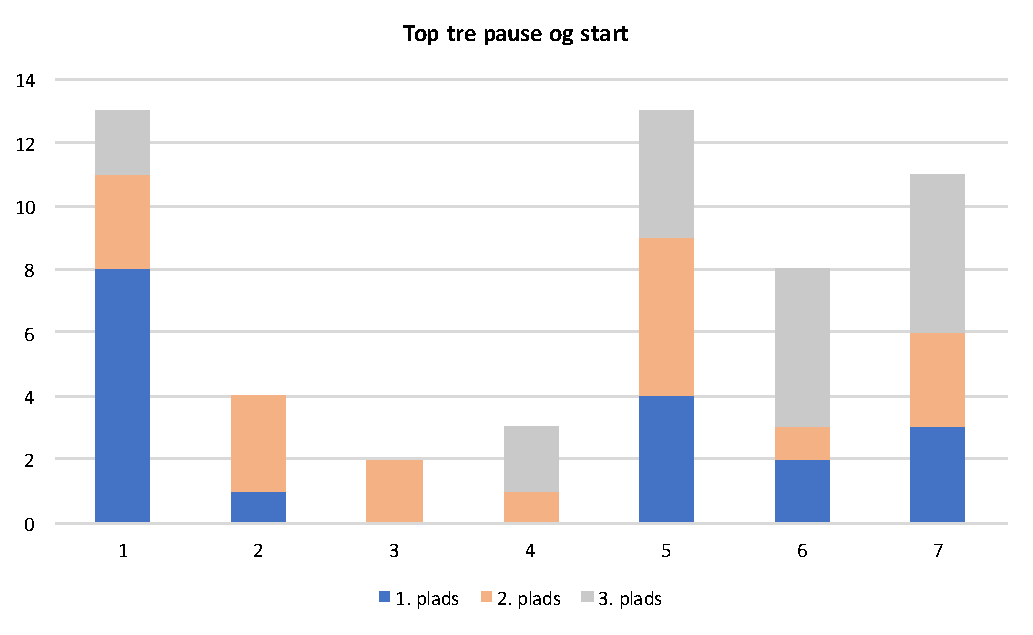
\includegraphics[resolution=300,width=0.9\textwidth]{Test1/DatabehandlingGrafer/TopTrePause}
	\caption{Søjlediagram over hvordan hvert gestik-par indgår i testpersonernes top tre i forhold til pause og start.}
	\label{fig:SamletTopTrePause}
\end{figure}
\noindent
%
Da der er tre gestik-par, som er blevet ekskluderet, kan ovenstående  \autoref{tab:GestikParITopTrePause} med fordel opsummeres både i forhold til at fjerne de tre gestik-par, men også i forhold til at opsummere, hvor mange gange de fire tilbageværende gestik-par indgår i top tre rangeringen. 
%
\begin{table}[H]
	\centering
	\begin{tabular}{ | p{2.4cm} | p{2.4cm} | p{2.4cm} | p{2.4cm} |p{2.4cm}|}
	\hline
		 & 1. Plads & 2. Plads & 3. Plads & I alt \\ \hline
		Gestik-par 1 & 8 & 3 & 2 & 13\\ \hline
		Gestik-par 5 & 4 & 5 & 4 & 13\\ \hline
		Gestik-par 6 & 2 & 1 & 5 & 8\\ \hline 
		Gestik-par 7 & 3 & 3 & 5 & 11\\ \hline
	\end{tabular}
	\caption{Oversigt over dels hvor mange gange hvert gestik-par indgår i samtlige testpersoners top tre i forbindelse med pause og start og dels over hvor mange gange et gestik-par sammenlagt indgår i en top tre.}
	\label{tab:GestikParITopTrePauseOversigt}
\end{table}
\noindent
% Gestik-par 1
Der er altså otte testpersoner, som alle rangerer gestik-par 1 på en førsteplads. Det tyder på at de otte testpersoner vurderer gestik-par 1 til at være en kombination af at være; simpel, enkel, logisk, naturlig, oplagt, nem at huske, nem at udføre, hurtig at udføre og vælger den, fordi den giver mening. Gestik-par 1 er illustreret på \autoref{fig:GestikPar1Pause}. Ud fra \autoref{tab:GestikParITopTrePause} fremgår det, at testperson 3 og testperson 10 har fuldstændig den samme top tre rangering og sammenholdes det med testpersonernes respons og videooptagelser, så er det også de eneste to testpersoner, som har gestik-par 1 på en første plads, som ikke er i tvivl om at gestik-par 1 skal være på en første plads. Når testperson 3 argumenterer for sin top tre, sker der på baggrund af udelukkelsesmetoden. Testpersonen nævner at gestik-par 5, gestik-par 6 og gestik-par 7 forbindes med en mute-funktion frem for en pause- og startfunktion. At forbinde gestikkerne med mute giver ikke nødvendigvis mening i denne sammenhæng, da det er ret usandsynligt at mute sin musik frem for at pause den, men i dette tilfælde danner det grundlag for testperson 3's top tre rangering. Testperson 10 giver udtryk for, at der, ved de gestik-par testpersonen har valgt, ikke er så stor risiko for, at testpersonen kommer til at lave dem anderledes og derudover er det ikke en bevægelse, som testpersonen hyppigt laver. Ifølge testperson 5, som har rangeret gestik-par 1 på en anden plads, så er bevægelsen; et statisik stop-tegn, jævnfør \autoref{fig:GestikPar1Pause}, normalt i ens kropssproget.   
%
\begin{figure}[H]
	\centering
	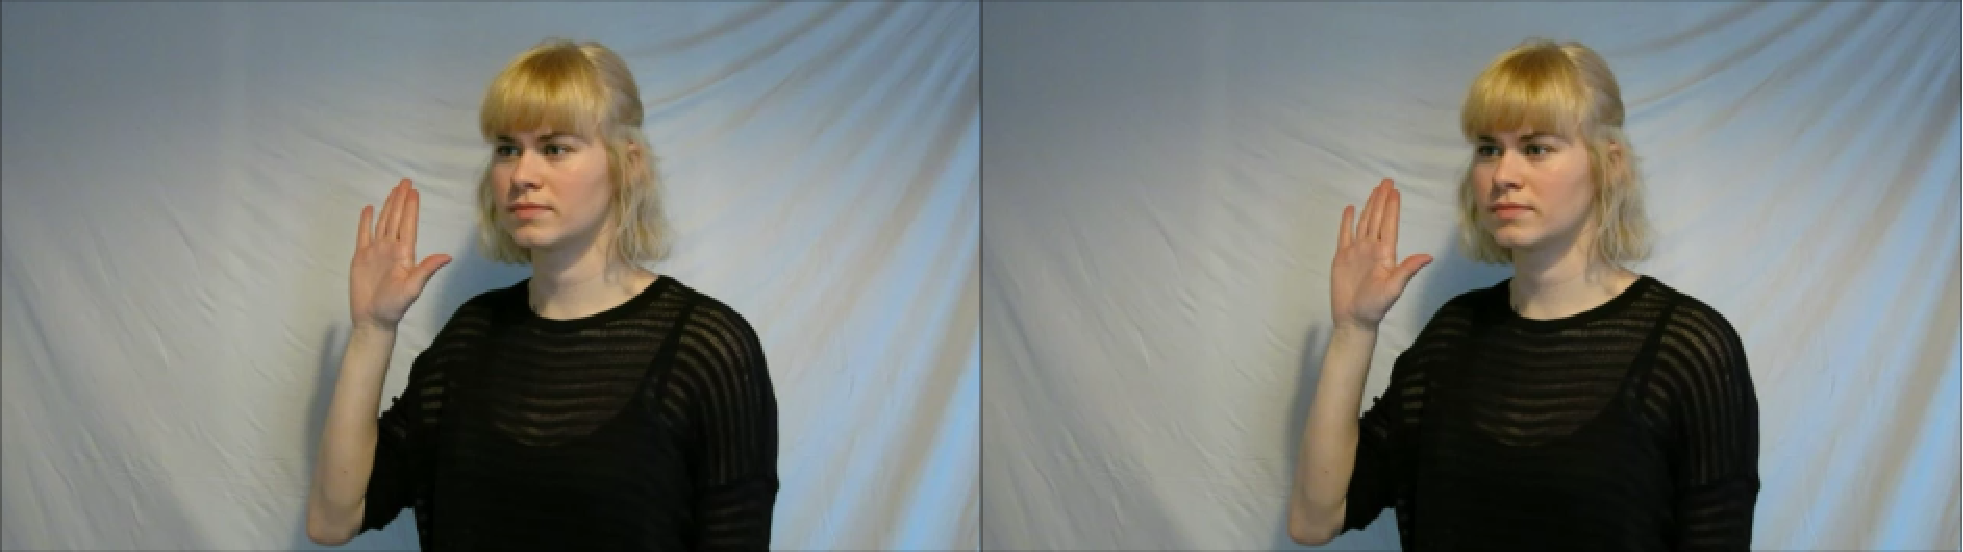
\includegraphics[resolution=300,width=0.9\textwidth]{Test1/Gestik-par/Gestik1_Pause}
	\caption{Illustration af gestik-par 1; stop-tegn til henholdsvis pause og start.}
	\label{fig:GestikPar1Pause}
\end{figure}
\noindent
% 	 
De seks andre testpersoner, som har rangeret gestik-par 1 på en første plads, har alle inkluderet gestik-par 5 enten på en anden plads eller en tredje plads. Testperson 1 svinger mellem at have gestik-par 1 og gestik-par 5 på en første plads, hvor testpersonen til at starte med har top tre rangeringen, der fremgår af \autoref{tab:GestikParITopTrePause}, hvorefter den ændres til; gestik-par 5, gestik-par 1 og gestik-par 7 på henholdvis en første, anden og tredje plads. Når testpersonen afslutningsvist skal gengive gestikkerne foretrækker testpersonen gestik-par 1 igen. På baggrund af det er det ikke muligt at afgøre, hvorvidt testperson 1's top tre rangeringen bør være gestik-par 1, gestik-par 5 og gestik-par 7 på henholdvis en første, anden og tredje plads, dog tyder det på at det er tilfældet. Ifølge testperson 16, er de tre gestik-par som testpersonen har rangeret i sin top-tre næsten lige gode, da de alle tre er simple, det tyder derfor på, at der ikke er stor forskel mellem en første, anden og tredje plads. Dog vurderer testpersonen, at gestik-par 1 er oplagt og den er ikke er til at glemme. Selvom testperson 4 ikke giver udtryk for at være i tvivl om sin top tre rangering, så tyder det på at testpersonen har rangeret gestik-par 1 højere end gestik-par 5, fordi gestik-parret er mere simpel. Dog giver testperson 4 udtryk for at gestik-par 5 er meget intuitiv. Ligende tendens forefindes ved testperson 17, som argumentere for hvorfor testpersonen har rangeret gestik-par 1 som værende den bedste; den er logisk. Når testperson 17 afslutningsvist bliver bedt om at gengive sine fortrukne gestikker, så er det gestik-par 5, som testpersonen knytter til pause og start. I og med at testpersonen tidligere har givet udtryk for, at gestikkerne skal falde testpersonen naturligt ind og at testpersonen ikke skal tænke over hvilken bevægelse der laves, så tyder det på at gestik-par 5 måske bør være rangeret over gestik-par 1.   

Selvom testperson 6 og testperson 15 har rangeret gestik-par 1 på en første plads, så tyder det på, at de foretrækker at der er bevægelse i gestikken. Testperson 6 gengiver, som en forbedring til gestik-par 1, en bevægelse, som minder om en kombination af gestik-par 1 og gestik-par 7, hvor håndens position fra gestik-par 1 bibeholdes mens fingrenes bevægelse i gestik-par 7 bibeholdes. Derudover giver testperson 6 også udtryk for, at mekanikken i gestik-par 5, hvor fingrene lukkes sammen for at pause og åbnes igen for at starte musikken, er god. Selvom det ikke nøjagtigt gengiver bevægelsen i gestik-par 5, så tyder det på, at det testperson 6 efterlyser formentlig kan opfyldes ved gestik-par 5. Testperson 15 giver udtryk for godt at kunne lide, at der er forskel på pause og start i gestik-par 5, hvilket ikke er tilfældet for de to gestik-par testpersonen har rangeret over gestik-par 5. 

Af de testpersoner, som har valgt gestik-par 1, er der, foruden testperson 6, kun to testpersoner, som har forbedringsforsalg. Testperson 4 foreslår, at hånden ikke behøver at være i en 90$^{\circ}$'s vinkel men istedet noget der minder om en 45$^{\circ}$ og derudover foreslår testpersonen, at det skal være ligegyldigt, hvor gestikken udføres; det må gerne være i hoftehøjde. Testperson 16 foreslår, at håndens position fastholdes i tre sekunder både for at pause og for at starte. Når testpersonen gengiver sin forbedring, så starter testpersonen med en knyttet næve, hvorefter fingrene foldes ud og danner et stop-tegn. Selvom testpersonen ikke eksplicit giver udtryk for det, så antages det, at dette ligeledes er en forbedring.
%
\begin{figure}[H]
	\centering
	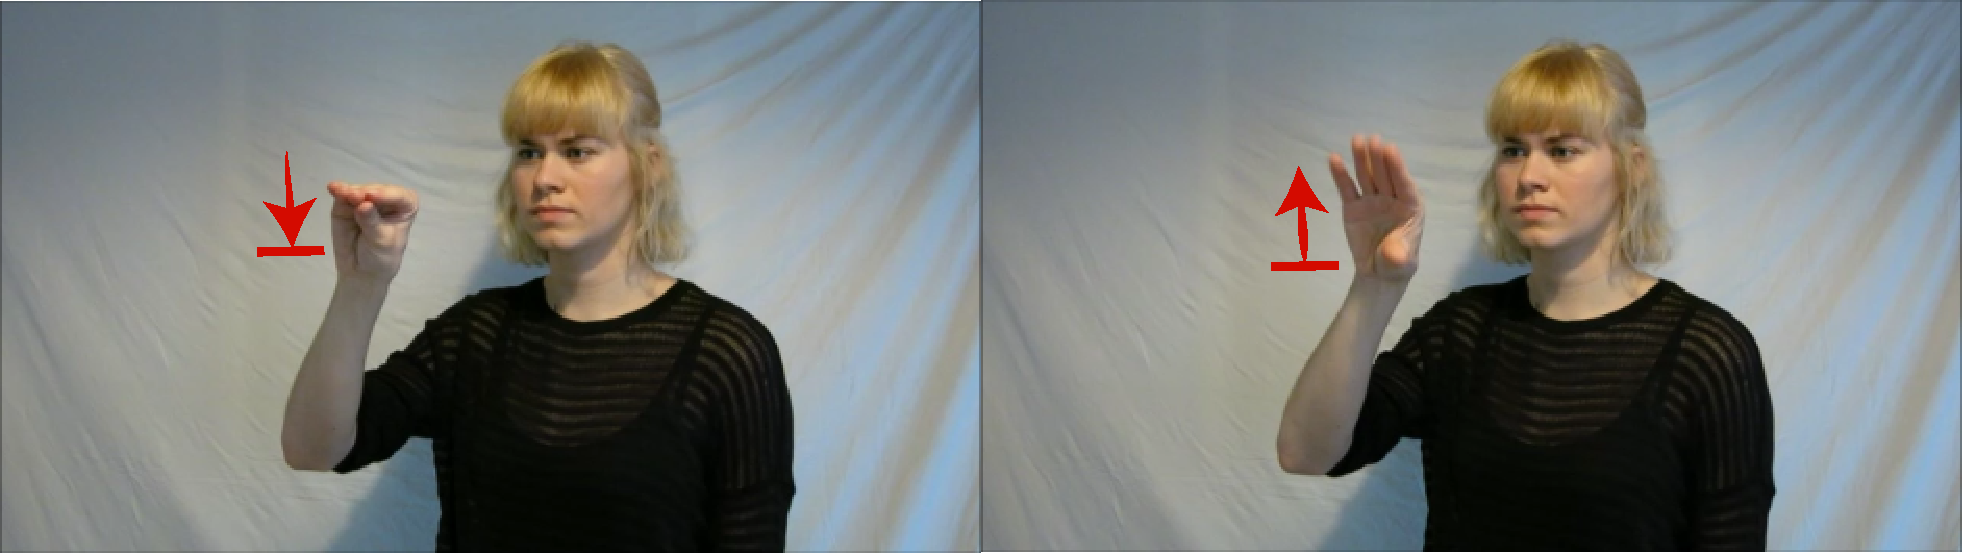
\includegraphics[resolution=300,width=0.9\textwidth]{Test1/Gestik-par/Gestik5_Pause}
	\caption{Illustration af gestik-par 5; krokodillenæb til henholdvis pause og start.}
	\label{fig:GestikPar5Pause}
\end{figure}
\noindent
% Gestik-par 5
Der er flere årsager til, at fire testpersoner har rangeret gestik-par 5 på en første plads, hvor den primære årsag er, at testpersonerne forbinder bevægelsen med en ti stille bevægelse, som de forbinder med at lukke munden på anlægget eller at de lukker musikken ned. Gestik-par 5 illustreres på \autoref{fig:GestikPar5Pause}. Testperson 18 pointerer, at det er en familiær bevægelse og at alle ved hvad det betyder, når en anden person laver luk-delen i et krokodillenæb til en; ti stille, jævnfør \autoref{fig:GestikPar5Pause}. Derudover er det ord som logisk, intuitiv og naturlig testpersonerne beskriver gestik-par 5 med. I relation til bevægelsen i gestik-par 5 så tyder det på, at testperson 5 favoriserer gestik-parret, fordi bevægelsen kan udføres tæt på kroppen og der skal ikke huskes et bestemt mønster. Derudover kommenterer testperson 11, at det er en lille bevægelse, faktisk den mindste bevægelse der kan laves, hvor det stadig giver mening. Testperson 11 giver ydermere udtryk for, at gestik-par 5 er det eneste gestik-par, som testpersonen egentligt bryder sig om, netop fordi det er en lille bevægelse. Testperson 7 har en anderledes tilgang til, hvorfor gestik-par 5 rangeres på en første plads. Testpersonen forestiller sig nemlig, at hvis interaktionen med musikanlægget vises frem for andre, så ville de syntes det var sjovt og de vil efterfølgende kunne det. Derudover giver testperson 7 også selv udtryk for, at gestik-par 5 er sjov. Foruden at gestik-par 5 er en familiær bevægelse, så giver testperson 18 ydermere udtryk for, at det er en gestik, som ikke laves ved en fejl. Testpersonen giver derudover udtryk for godt at kunne lide, at der er forskel på, hvordan musikken pauses og startes igen, med henholdvis en luk- og åben bevægelse. Testperson 1, der som nævnt flere gange skifter mening om sin første prioritet, giver udtryk for godt at kunne lide gestik-par 5, fordi det giver mening i forhold til at skrue op og ned for musikken, hvilket er testpersonens argumentation for at den også passer til at pause og starte musikken.

Af de fire testpersoner, som har valgt gestik-par 5, er der to testpersoner, som har forbedringsforslag. Testperson 5 foreslår ingen ændringer til at pause musikken, men når musikken startes igen foreslår testpersonen, at hånden udadroterer som krokodillenæbet åbnes, hvilket resulterer i at slutpositionen er med tommelfingeren øverst. Selvom forslaget i sig selv er fint, så forventes det, at når musikken er blevet sat på pause, så skal hånden selvfølgelig ikke fastholdes i det lukkede krokodillenæb, illustreret på \autoref{fig:GestikPar5Pause}, men kunne bevæges frit. Når hånden, afslappet, frigøres fra krokodillenæbet så kan det for nogen være meget naturligt at lave en bevægelse, som minder om testperson 5's forbedringsforslag til at starte musikken, hvorfor dette forbedringsforslag afvises. Forbedringsforslaget fra testperson 18 kan nærmere betragtes som en selvfølge end en decideret forbedring. Testpersonen foreslår nemlig, at gestikken ikke behøver at blive lavet i hovedhøjde, men bør kunne laves over alt. Grunden til at forbedringsforslaget anses som værende en selvfølge, er fordi det bør gøre sig gældende for samtlige semaforiske gestikker, at de ikke defineres ud fra en bestemt højde, men frit kan udføres.
%
\begin{figure}[H]
	\centering
	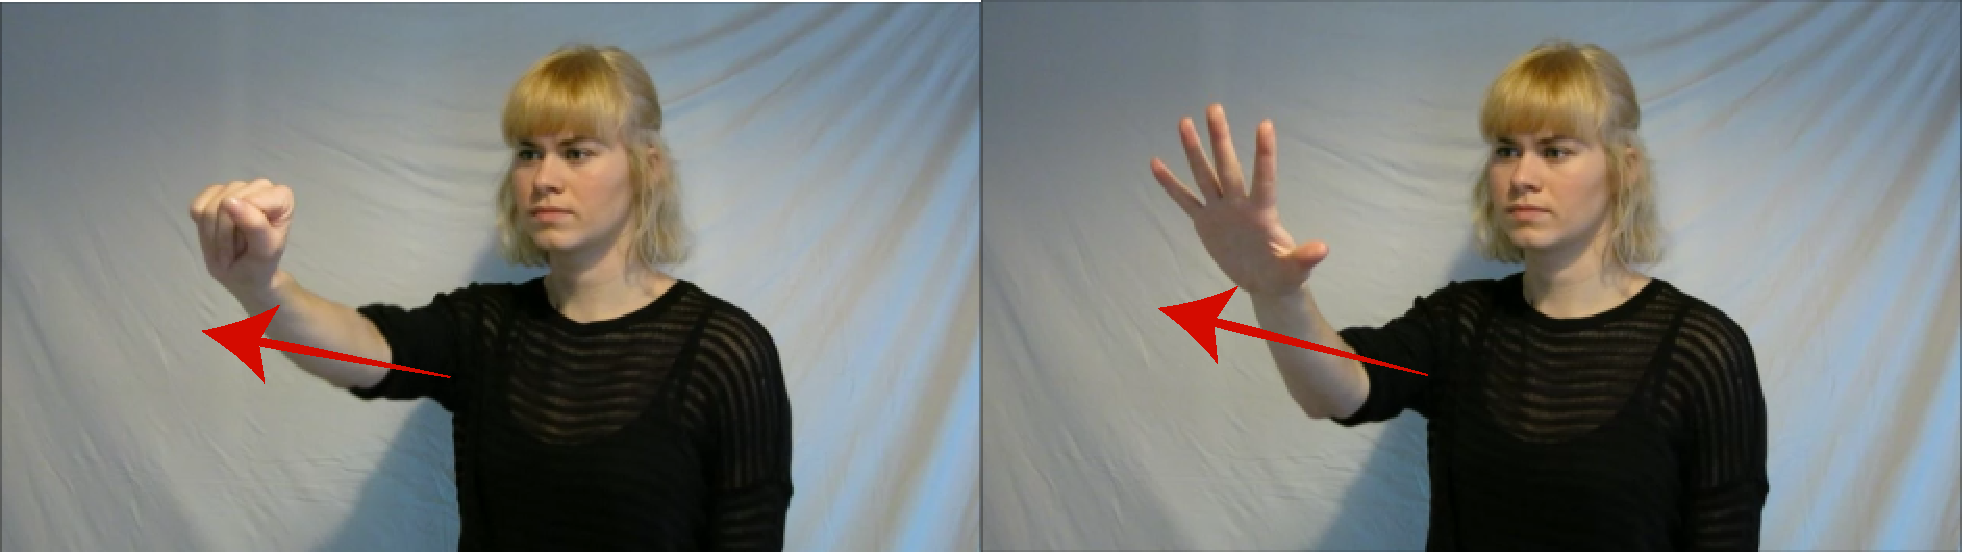
\includegraphics[resolution=300,width=0.9\textwidth]{Test1/Gestik-par/Gestik6_Pause}
	\caption{Illustration af gestik-par 6; hånden lukker sammen i en dynamisk horisontal bevægelse til pause og hånden åbner i en dynamisk horisontal bevægelse til start.}
	\label{fig:GestikPar6Pause}
\end{figure}
\noindent
% Gestik-par 6
Ud af 18 testpersoner, er der kun to testpersoner; testperson 13 og testperson 14, som har gestik-par 6 rangeret på en første plads. Gestik-par 6 illustreres på \autoref{fig:GestikPar6Pause}. Baseret på testperson 13's udsagn, kan det ikke udledes, hvorfor testpersonen foretrækker gestik-par 6, hvilket skyldes, at indtil testpersonen opfordres til at komme med et forbedringsforslag, så er det gestik-par 3, som testpersonen foretrækker. Dog kommenterer testperson 13, at det ikke er muligt at afgøre hvilket gestik-par, der er bedst af gestik-par 6 og gestik-par 7 fordi den eneste forskel er, hvilken retning bevægelsen foregår i. Ifølge testperson 14 vælges gestik-par 6, fordi det er tilpas akavet samtidig med, at det er en naturlig bevægelse i forhold til at skulle åbne og lukke lyd. Derudover pointere testpersonen at det giver god meningen, at bevægelsen rettes mod musikanlægget. Da der kun er to testpersoner, som har rangeret gestik-par 6 på en første plads og gestik-parret sammenlagt kun indgår otte gange i testpersonernes samlede top tre rangering, samt at flere testpersoner giver udtryk for, at de åbne omkring deres anden og tredje plads, så vurderes det at der er belæg for at ekskludere gestik-par 6. 
%
\begin{figure}[H]
	\centering
	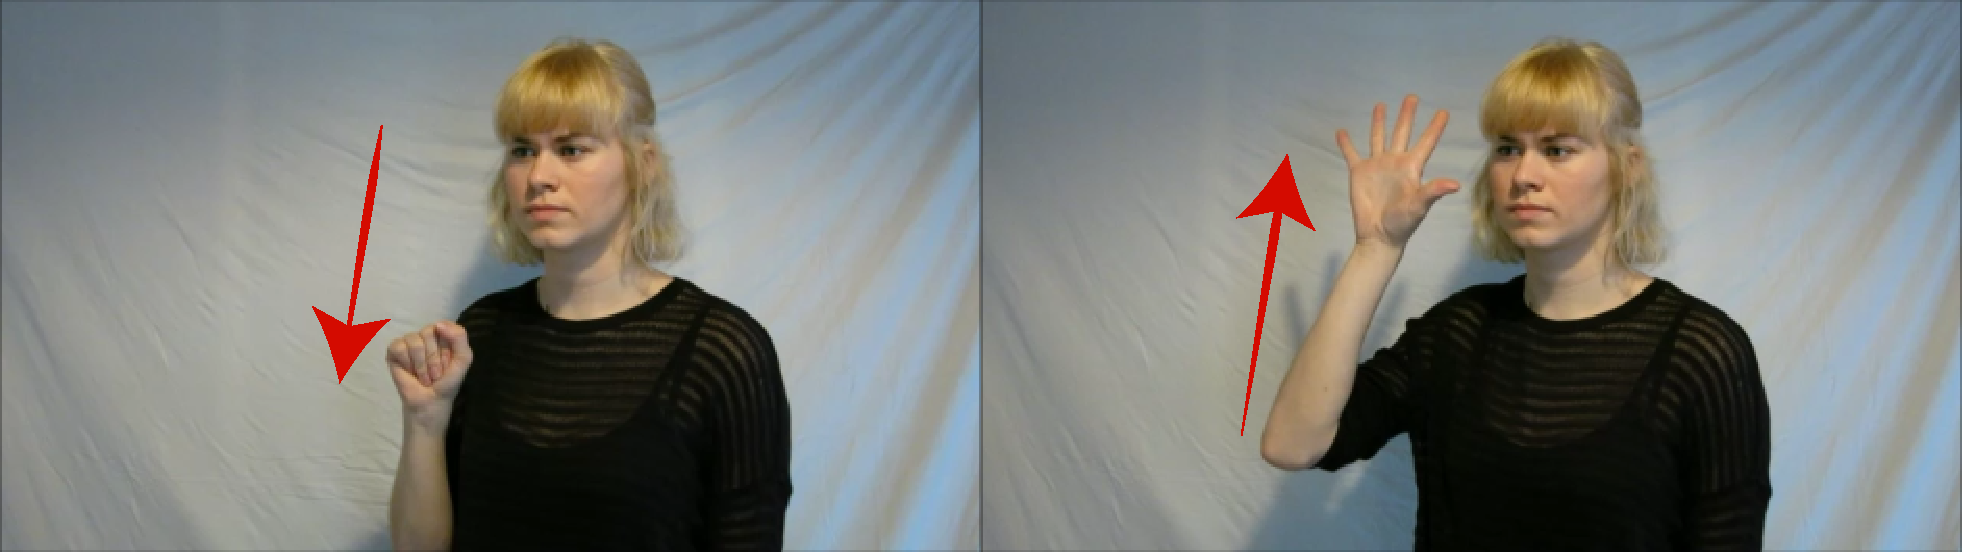
\includegraphics[resolution=300,width=0.9\textwidth]{Test1/Gestik-par/Gestik7_Pause}
	\caption{Illustration af gestik-par 7; hånden lukker sammen i en dynamisk vertikal bevægelse nedad til pause og hånden åbner i en dynamisk vertikal bevægelse opad til start.}
	\label{fig:GestikPar7Pause}
\end{figure}
\noindent
% Gestik-par 7
Baseret på de tre testpersoner, som har tildelt gestik-par 7 en første plads, tyder det på at testperson 2 har valgt gestik-par 7, fordi det er en simpel bevægelse, som giver meget mening og fordi der er forskel på pause og start. Gestik-par 7 illustreres på \autoref{fig:GestikPar7Pause}. Det er begrænset hvad der kan udledes af testperson 8, da testpersonen til at starte med rangerer gestik-par 3 på en første plads. Det kan dog udledes, at gestik-par 7 giver mening. Det er svært at udlede noget konkret ud fra testperson 9's udsagn, dog virkede det, ifølge testperson 9, logisk at skulle gribe ud efter musikken for at pause den og slippe musikken fri for at starte musikken igen. Da det er begrænset hvad der kan udledes fra de tre testpersoner, som har gestik-7 på en første plads og at gestik-par 7 trods alt sammenlagt indgår 11 gange i den samlede top tre, så vurderes det, at det er nødvendigt at inddrage de otte testpersoner, som har inkluderet gestik-par 7 i deres top tre. 

De tre testpersoner, som har rangeret gestik-par 7 på en anden plads, er testperson 1, testperson 11 og testperson 18. Alle tre testpersoner giver udtryk for, at bevægelsen giver mening i forhold til at pause musikken ved at trække ned og starte musikken igen ved den modsatte bevægelse, jævnfør \autoref{fig:GestikPar7Pause}. Derudover pointerer testperson 1, at bevægelsen er forholdvis enkel og den er nem at huske. Testperson 11 kommenterer at det er intuitivt, hvordan musikken lukkes ned og testperson 18 vurderer, at det ikke er en bevægelse, der laves ofte. Det skal understreges at kommentarerne fra testperson 11 primært bygger på, hvad testpersonen giver udtryk for i forhold til gestik-par 5. At de indgår her, skyldes at testpersonen giver udtryk for at både gestik-par 6, illustreret på \autoref{fig:GestikPar6Pause}, og gestik-par 7, illustreret på \autoref{fig:GestikPar7Pause}, minder meget om gestik-par 5, illustreret på \autoref{fig:GestikPar5Pause}, hvorfor det vurderes at disse kommentarer ligeledes relaterer sig til gestik-par 7. Baseret på begrundelserne fra de fem testpersoner, som har tildelt gestik-par 7 en tredje plads, så tyder det på at det primært er fordi bevægelsen følge samme bevægelsesmønster, som enten den ene eller begge de par, som testpersonerne har rangeret højere. Fra \autoref{tab:GestikParITopTrePause} fremgår det, at hver gang en testperson tildeler gestik-par 7 en tredje plads, så tildeles anden pladsen altid gestik-par 5. Ligende tendens går igen, når gestik-par 7 tildeles en anden plads, hvor to ud af tre testpersoner har tildelt gestik-par 5 en første plads. Hvis gestik-par 7 derimod indgår på en første plads, så er der ingen af de tre testpersoner, som inkluderer gestik-par 5, til gengæld inkluderer de gestik-par 1, gestik-par 3 og gestik-par 6. 

Da det tyder på, at testpersonerne i højere grad foretrækker enten gestik-par 1, illustreret på \autoref{fig:GestikPar1Pause}, eller gestik-par 5, illustreret på \autoref{fig:GestikPar5Pause}, over gestik-par 7, illustreret på \autoref{fig:GestikPar7Pause}, samtidig med at gestik-par 5 indeholder to forskellige bevægelser til henholdvis pause og start, som er noget testpersonerne, der har inkluderet gestik-par 7, efterspørger, så vurderes det at der er belæg for at ekskludere gestik-par 7. \blankline
% Udvælgelse af gestik-par til at pause og starte musikken
Baseret på foregående analyse samt \fullref{app:TestresultaterPauseDaarlig}, hvor i alt fem gestik-par er ekskluderet, så står valget mellem gestik-par 1 og gestik-par 5. Fælles for de to gestik-par er, at de indgår lige mange gange i testpersonernes samlede top tre; 13 gange i alt, selvom gestik-par 1 er tildelt en første plads dobbelt så mange gange som gestik-par 5. Det tilstræbes at imødekomme så mange testpersoners ønske, som muligt, og flere testpersoner giver udtryk for at foretrække dels, at der er bevægelse og dels, at der er forskel påhvordan musikken sættes på pause og hvordan den startes igen, hvilket opnås i gestik-par 5. Derudover er risikoen for at lave gestik-par 5, ved en fejl, mindre end ved gestik-par 1. At gestik-par 1 af flere testpersoner beskrives, som værende en naturlig bevægelse, er ikke nødvendigvis et godt argument for at vælge den gestik, da stop-tegnet kan opstå i urelaterede situationer. Endvidere har seks ud af de otte testpersoner, som har tildelt gestik-par 1 en første plads, også inkluderet gestik-par 5 i deres top tre og fire ud af de seks har tildelt parret en anden plads. Tages alt dette i betragtning vurderes det at der findes tilstrækkeligt belæg for at knytte gestik-par 5 til pause og start.            





